
\documentclass[12pt,a4paper]{scrartcl}

\usepackage{mystyle}

\loadglsentries[main]{tex/glossar}
\makeglossaries%Glossar
\makeindex

\title{Entwicklung einer mobilen Webanwendung zur Planung und Unterstützung von Open Spaces.}
\author{Christoph Hegemann}

\begin{document}
\maketitle
\clearpage
%\newcommand{\doublesignature}[2]{%
    \parbox{7cm}{
      \rule{6cm}{1pt}\\
      #1
    }
    \hfill
    \parbox{7cm}{
      \rule{6cm}{1pt}\\
      #2
    }
  }
%%% Local Variables:
%%% mode: latex
%%% TeX-master: "../Doku"
%%% End:

\pagenumbering{roman}
\section{Projektantrag}
\section*{Projektbezeichnung/Auftrag/Teilauftrag}
Entwicklung einer mobilen Webanwendung zur Planung und Unterstützung
von Open Spaces.
\subsection*{Ausgangssituation}
Die als Auftraggeber auftretende OPITZ CONSULTING Deutschland GmbH ist
ein mittelständisches, wachsendes Unternehmen im Bereich der
IT-Beratung und Dienstleistung. Am Hauptsitz in Gummersbach befindet
sich neben der Holding Gesellschaft noch der Größte der insgesamt neun
Standorte.

\noindent Seit einigen Jahren werden bei Opitz regelmäßig Open Spaces durchgeführt.
Ein Open Space ist eine Veranstaltung, bei der mehrere Personen
zusammen kommen, Themen vorschlagen und diese in einer wie auch immer
gearteten Weise bearbeiten, besprechen oder erlernen. Ein Open Space
verteilt sich hierbei auf mehrere Räume und Timeslots, die zuvor
festgelegt werden müssen. Die Themen werden von den Teilnehmern selbst
angeboten und die Teilnehmer entscheiden mit ihrer Interessenbekundung
an einem oder mehreren Themen, wie sich das Programm gestaltet.
(siehe auch:\footnote{\url{http://en.wikipedia.org/wiki/Open_Space_Technology}})
Falls die Teilnehmer nach Ablauf der Zeit eines Themas weiteres
Interesse anmelden kann das Thema ad hoc verlängert und verlegt werden.

\noindent Derzeit verläuft die Planung dieser Open Spaces direkt auf
der Veranstaltung mithilfe von Whiteboards oder Flipcharts. Im
Nachhinein wird dann zumeist in einem CMS über die Veranstaltungen
berichtet und Bilder hochgeladen, wobei dies auf freiwilliger Basis
geschieht und zusätzlichen Aufwand bedeutet.

\noindent Dieses sehr statische Planungsvorgehen wird dem dynamischen
Charakter von Open Spaces nicht gerecht. Als verteilte Veranstaltung
mit ``Realtime''-Aspekt ist für eine sinnvolle Kommunikation ein hohes
Maß an Vernetzung unverzichtbar. Das dokumentieren der parallelen und
verteilten Vorgänge ist aus der Sicht einer Person aufwendig und das
Ergebnis lückenhaft. Eine mobile Webanwendung kann und soll hier
Abhilfe schaffen.
\subsection*{Zielsetzung}
Ziel des Projektes ist es, eine erweiterbare Full-Stack-Anwendung zu
entwickeln, welche die Durchführung von Open Spaces unterstützt. Der
Veranstaltungscharakter legt den Anwendungsfall nahe, eine Instanz
dieser Applikation bei Bedarf zu starten und nach der Durchführung der
Veranstaltung wieder zu beenden. Hieraus lässt sich die Cloud als
geeignete Plattform ableiten. Eine weitere Anforderung an die
Anwendung ist ein mobiler Client, der den Teilnehmern eine Sicht auf
den aktuellen Zeitplan und die Aufnahme und Verteilung von Bildern und
Notizen ermöglicht. Außerdem sollen über den mobilen Client in einem
Push-basierten Modell Notifikationen über Änderungen am Zeitplan
verteilt werden.
Ein weiteres Ziel ist die Evaluierung von funktionalen
Programmiertechniken im Bezug auf ihre Tauglichkeit für die Erstellung
von Webapplikationen.
\subsection*{Konsequenzen bei Nichtverwirklichung}
Open Spaces werden weiterhin am Whiteboard geplant und Änderungen am
Zeitplan erreichen  Teilnehmer nur dann, wenn diese am zentralen Board
nachgetragen werden und die Teilnehmer sich dort regelmäßig über
Änderungen informieren. Die Dokumentation des zeitlichen Ablaufs
gestaltet sich weiterhin als schwierig.
\section*{Projektumfeld/Rahmenbedingungen}
Um möglichst viele Plattformen (Windows, MacOS, Linux, iOS, Android)
und Geräte (Dekstop, Mobile Endgeräte) ansprechen zu können, soll die
Entwicklung der Anwendung auf Webtechnologien basieren. Als
Versionierungsmodell soll ein Continuous Integration System aufgesetzt
werden.
\section*{Projektplanung}
\subsubsection*{Zeitplanung}
\begin{tabular}{l l r}
1. & Planung & 2h \\
2. & Entwurf & 5h \\
\toprule 3. & Implementierung & \\
3.1 & Browser Frontend & 15h \\
3.2 & Backend & 20h \\
3.3 & Mobile Webapp & 5h \\
\toprule 4. & Abschließender Test & 5h \\
5. & Übergabe & 3h \\
6. & Dokumentation & 15h \\
\toprule $\Sigma$ & Summe & 70h
\end{tabular}

\section*{Anzufertigende Dokumente}
\begin{itemize}
\item Projektdokumentation
\item Selbstständigkeitserklärung
\item Screenshots der Anwendung
\item Quellcode
\end{itemize}

\section*{Erklärungen}
\subsection*{Erklärung des Prüfungsteilnehmers}
Ich versichere durch meine Unterschrift, dass ich das Projekt und die dazugehörige Dokumentation
selbständig und ohne fremde Hilfe angefertigt und alle Stellen, die ich wörtlich oder annähernd
wörtlich aus Veröffentlichungen entnommen habe, als solche kenntlich gemacht habe. Die Arbeit
hat in dieser Form keiner anderen Prüfungsinstitution vorgelegen.\\[1.5cm]
%\doublesignature{Ort, Datum}{Unterschrift des Prüfungsteilnehmers}
\subsection*{Erklärung des Ausbildungsbetriebes}
Wir versichern, dass das Projekt wie in der Dokumentation dargestellt, in unserem Unternehmen
realisiert worden ist.\\[1.5cm]
%\doublesignature{Ort, Datum}{Unterschrift des Ausbilders}
\section*{Sperrvermerk}
Die vorliegende Abschlussarbeit mit dem Titel ``Entwicklung einer mobilen Webanwendung zur Planung und Unterstützung von Open Spaces'' enthält vertrauliche Daten des Unternehmens OPITZ CONSULTING Deutschland GmbH.
\\[0.5cm]
Die Abschlussarbeit darf nur dem Erst-  und Zweitgutachter sowie  befugten Mitgliedern des
Prüfungsausschusses zugänglich gemacht werden. Eine Veröffentlichung und Vervielfältigung
der Abschlussarbeit ist \- auch in Auszügen \- nicht gestattet.
\\[0.5cm]
Eine Einsichtnahme der Arbeit durch Unbefugte bedarf einer ausdrücklichen Genehmigung des
Verfassers und des Unternehmens OPITZ CONSULTING Deutschland GmbH.

\tableofcontents
\listoffigures
%\listoftables
\clearpage
\pagenumbering{arabic}
\section{Ausgangssituation}
\subsection{Unternehmensbeschreibung}
Das IT-Beratungshaus OPITZ CONSULTING Deutschland GmbH ist ein
wachsendes, mittelständisches Unternehmen im Bereich der IT-Beratung
und -Dienstleistung. Am Hauptsitz in Gummersbach befinden sich die
Holding-Gesellschaft sowie der Größte der insgesamt neun Standorte.
Das Unternehmen ist seit seiner Gründung im Jahr 1990 auf derzeit etwa
400 Mitarbeiter gewachsen. Die 9 Standorte setzen sich aus sieben
Standorten in Deutschland, sowie zwei Standorten in Polen zusammen.
\subsection{Projekthintergrund}
Seit einigen Jahren werden bei OPITZ-CONSULTING regelmäßig Open Spaces
durchgeführt. Ein Open Space ist eine Veranstaltung, bei der mehrere
Personen zusammen kommen, Themen vorschlagen und diese in einer wie
auch immer gearteten Weise bearbeiten, besprechen oder erlernen. Ein
Open Space verteilt sich hierbei auf mehrere Räume und Timeslots, die
zuvor festgelegt werden müssen. Die Themen werden von den Teilnehmern
selbst angeboten und die Teilnehmer entscheiden mit ihrer
Interessenbekundung an einem oder mehreren Themen, wie sich das
Programm gestaltet. (siehe auch:\footnote{\url{http://en.wikipedia.org/wiki/Open_Space_Technology}})
Falls die Teilnehmer nach Ablauf der Zeit eines Themas weiteres
Interesse anmelden kann das Thema ad hoc verlängert und verlegt
werden.
\noindent Derzeit verläuft die Planung dieser Open Spaces direkt auf
der Veranstaltung mithilfe von Whiteboards oder Flipcharts. Im
Nachhinein wird dann zumeist in einem \gls{CMS} über die Veranstaltungen
berichtet und Bilder hochgeladen, wobei dies auf freiwilliger Basis
geschieht und zusätzlichen Aufwand bedeutet.

\noindent Dieses sehr statische Planungsvorgehen wird dem dynamischen
Charakter von Open Spaces nicht gerecht. Als verteilte Veranstaltung
mit ``Realtime''-Aspekt ist für eine sinnvolle Kommunikation ein hohes
Maß an Vernetzung unverzichtbar. Das dokumentieren der parallelen und
verteilten Vorgänge ist aus der Sicht einer Person aufwendig und das
Ergebnis lückenhaft. Eine mobile Webanwendung kann und soll hier
Abhilfe schaffen.

%%% Local Variables:
%%% mode: latex
%%% TeX-master: "../Doku"
%%% End:

\section{Projektplanung}
\subsection{IST-Analyse}
Auf die aktuelle Lage wurde bereits ausreichend in der Beschreibung
der Ausgangssituation eingegangen. Darum sollen hier nur noch einmal
die wichtigsten Punkte aufgelistet werden.
\begin{itemize}
\item Es gibt eine vorhandene Lösung für das Zusammentragen von Themen
  im Voraus
\item Fehlende Möglichkeit während des Open Spaces Änderungen am
  Zeitplan vorzunehmen
\item Fehlende Möglichkeit diese Änderungen in Echtzeit an die
  Teilnehmer weiter zu reichen
\item Fehlende Möglichkeit für das Festhalten der Ergebnisse der
  durchgeführten Diskussionen, Workshops, etc\ldots
\end{itemize}
\subsection{SOLL-Konzept}
Gewünscht ist eine Möglichkeit die zuvor gesammelten Themenvorschläge
auf Räume und Zeitslots zu verteilen. Weiterhin soll es möglich sein
neue Themen hinzuzufügen. Der Zeitplan muss sich in Echtzeit anpassen
lassen und die vorgenommenen Änderungen sollen alle Teilnehmer des
Open Spaces erreichen. Als zusätzliche Anforderung soll die gewünschte
Applikation in einem funktionalen Stil entwickelt werden um spätere
Änderungswünsche leichter umsetzen zu können. Dieser Effekt soll sich
durch das Vermeiden von Seiteneffekten, sowie Modularisierung und das
Programmieren mit Unveränderlichen Variablen einstellen.
\subsection{Zielsetzung}
Primärziel ist es eine Webapplikation zur Unterstützung von Open
Spaces zu entwickeln. Weitere Ziele sind eine mobile Lösung um den
Zeitplan zu betrachten sowie die Tauglichkeit von funktionalen
Techniken für die Webentwicklung zu evaluieren.
\subsection{Infrastrukturelle Rahmenbedingungen}
Für die Applikation wird ein Server zur Verfügung gestellt. Die
Administration dieses Servers geschieht über \gls{ssh}. Der Server
wird zeitlich begrenzt für die Dauer des Open Spaces bereitgestellt.
\subsubsection{Entwicklungsumgebung}
Entwickelt wurde auf einem Ubuntu 14.04 Linux System. Als
Entwicklungsumgebung diente Emacs mit Plugins für den jeweiligen
Einsatzfall. Die Applikation wurde mit Chrome und Firefox auf dem
angesprochenen Linux System getestet. Während der Entwicklung wurden
der Server sowie die Datenbank lokal betrieben.
\subsubsection*{Verwendetes Tooling am Backend:}
\begin{itemize}
\item \gls{ghc} in Version \texttt{7.8.3}
\item \gls{cabal} in Version \texttt{1.20.0.0}
\item \gls{postgresql} in Version \texttt{9.3.6}
\end{itemize}

\subsubsection*{Verwendetes Tooling am Frontend:}
\begin{itemize}
\item \gls{psc} in Version \texttt{0.6.8}
\item \gls{react-tools} in Version \texttt{0.12.2}
\item \gls{pulp} in Version \texttt{2.0.2}
\item \gls{bower} in Vesion \texttt{1.3.5}
\end{itemize}
Es wurde außerdem ein Buildserver in einer Virtuellen Maschine
aufgesetzt, der die spätere Laufzeitumgebung für den Server
nachbildet. Auf diesem Buildserver gebaute Programme können einfach
auf das Produktivsystem kopiert und dort benutzt werden.
\subsubsection{Laufzeitumgebung}
Das entwickelte Backend soll abschließend auf einem Debian Server
laufen. Die Webapplikation (das Frontend) soll sowohl im Browser auf
Desktop Clients, als auch in den Browsern der mobilen Clients
ausgeführt werden.
\subsection{Terminplanung}
Das Projekt ist zwischen dem 25.01.2015 und dem 17.04.2015 zu
realisieren und umfasst maximal 70 Arbeitsstunden.

%%% Local Variables:
%%% mode: latex
%%% TeX-master: "../Doku"
%%% End:

\section{Realisierung}
\subsection{Vorgehensweise}
Als Vorgehensweise wurde das erweiterte
Wasserfall-Modell gewählt. (Abbildung~\ref{fig:wasserfall_modell})
\begin{figure}[h]
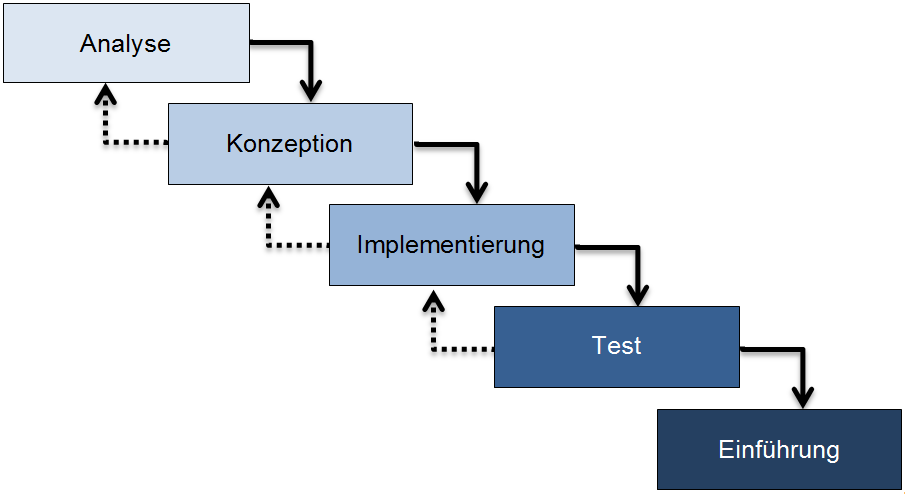
\includegraphics[scale=0.5]{img/wasserfall_modell.png}
\caption{Erweitertes Wasserfallmodell\label{fig:wasserfall_modell}}
\end{figure}

\noindent Aufgrund der knappen Zeitanforderungen bietet ein solcher Ansatz
den Vorteil eines direkten, klaren Pfades vom Beginn zum Ende des
Projektes. Im erweiterten Wasserfall-Modell erhält man, durch die
Möglichkeit kleine Rückschritte zu machen, die nötige Flexibilität um
auf Feedback einzugehen und Dinge ausprobieren zu können.
\subsection{Analyse \& Konzeption}
Bei der Analyse der Anforderungen fallen die Realtime Aspekte auf. Sie
sollen mithilfe von Websocketkommunikation und Push-Based-Updates vom
Server umgesetzt werden. Für einen modernen Look und ein intuitives
Verhalten soll die Steuerung Drag and Drop unterstützen.
\subsubsection*{Architektur}
Zu Beginn wurde ein Plan für das grobe Zusammenspiel der beteiligten
Komponenten angefertigt. Hiermit wurde die Arbeit in mehrere Schritte
und leicht abzugrenzende Komponenten unterteilt. Das Projekt ließ sich
damit in Meilensteine aufteilen, um strukturiert an das Projekt
herangehen zu können.

Die Architektur gibt dabei folgende Aufteilung her:
\begin{itemize}
\item Datenbank
\item Backend Server
\item Desktop Frontend
\item Mobile Frontend
\end{itemize}
Einen Überblick über die spätere ``physikalische Ausprägung'' des
Systems soll Abbildung~\ref{fig:architektur} geben.
\begin{figure}[h]
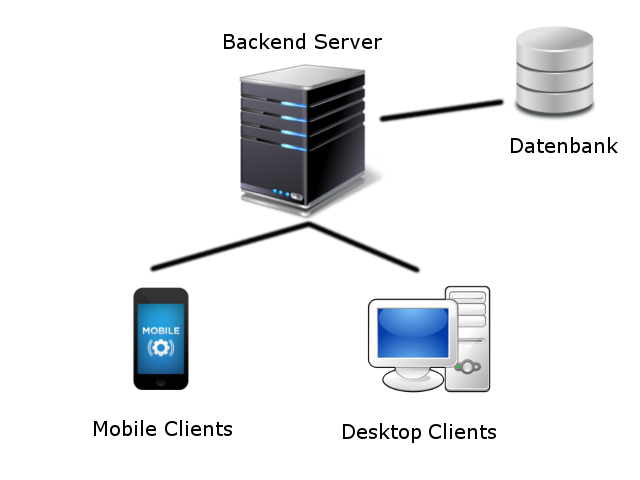
\includegraphics[scale=0.5]{img/Architektur.png}
\caption{Architektur Übersicht\label{fig:architektur}}
\end{figure}
Die Clients (Mobile / Desktop) kommunizieren über WebSockets mit dem
Backend-Server. Dieser speichert und liest Daten aus einer Datenbank.
Durch die WebSockets ist es dem Backend-Server möglich Änderungen am
Datenmodell mittels Push-Benachrichtigungen an die Clients weiterzugeben.
\subsection{Implementierung}
\subsubsection{Browser-Frontend}
Die Implementierung des Browser-Frontends verwendet Technologien, die
dem \gls{Reactive Programming} Pattern zuzuweisen sind. \gls{React} als
UI-Framework von Facebook ist ein stark durch funktionale Ideen und
\gls{Reactive Programming} inspiriertes Framework. Dies bedeutet
konkret, dass die elementaren Objekte der Programmierung keine
skalaren Werte wie Numbers oder Strings sondern Streams von
solchen sind. Dies erlaubt es, Werte die sich über die Zeit verändern,
in einem deklarativen Stil zu beschreiben und angemesssene
Abstraktionen für Echtzeitsysteme zu finden. \gls{Reactive
  Programming} ermöglicht außerdem besonders kurze Antwortzeiten auf
Nutzerinteraktion, was zu einem besseren Nutzererlebnis führt. Die
Applikation leidet nicht unter Ladezeiten und reagiert schnell und
zuverlässig.

Das Browser Frontend ist modular aufgebaut, wobei das Modulsystem von
\gls{PureScript} behilflich ist. Ein Modul kapselt dabei die
Definitionen innerhalb einer Datei und kann von anderen Modulen
importiert werden. Dies erlaubt es das Dateisystem zu nutzen um Teile
des Systems inhaltlich voneinander abzugrenzen. Das Prinzip von der
starken Kohäsion und losen Kopplung ist ein wichtiges Ziel bei der
Architektur und dem Design von Software und lässt sich mithilfe des
Modulsystems von PureScript leichter umsetzen.

Die Kommunikation mittels WebSockets und das Verwalten des
Applikationszustandes geschieht in der in \gls{PureScript}
implementierten Engine. Dieser Teil des Programmes nimmt im
Unidirectional-Dataflow Modell die Rolle der ``Stores'' ein und
erlaubt es das View-Layer beliebig auszutauschen. Die Engine ist für
alle Clients gleich und kann daher für die mobile Version des Clients
wiederverwendet werden.

\begin{figure}[h]

\includegraphics[scale=0.3]{img/Unidirectional.png}
\caption{Unidirectional Dataflow}
\end{figure}

\noindent Die Engine ``pusht'' den Applikationszustand in das
View-Layer, welches aus diesem ein User Interface rendert.
Die Interaktionen des Benutzers mit dem View-Layer erzeugen dann
wiederum Events, die als Streams an die Engine zurückfließen, wo sie
interpretiert und verarbeitet werden. Das Interpretieren der Events
lässt sich, dank des deklarativen Stils den PureScript erlaubt, leicht
programmieren. Als Beispiel soll der Code dienen, der das Ziehen eines
Themas auf das Grid beschreibt.

\begin{lstlisting}
  dragTopic = do
    Right t <- dragStart
    action <- dragOver
    lookup "dragEndTopic" `merge` lookup "dragEndGridTopic"
    return $ action t
\end{lstlisting}
\noindent Hier werden die Eventstreams für den Beginn eines
Drag Vorgangs sowie das Ziehen über einen Zeitslot mit dem Beenden des
Drag Vorgangs kombiniert und in einem resultierenden Stream \texttt{dragTopic}
ausgegeben. Dieser Stream abstrahiert nun die Mechanik des Drag and
Drop Vorganges und erlaubt es die tatsächlichen Intentionen des
Nutzers zu modellieren, um angemessen auf diese reagieren zu können.
\subsubsection{Backend Server}
Für die Entwicklung des Backend Servers wurde Haskell als
Programmiersprache ausgewählt. Haskell ist eine rein funktionale
Sprache und bringt dadurch die schon angesprochenen Vorteile im Bezug
auf Modularität und Skalierbarkeit mit sich. Die Implementierung
verwendet das \gls{Yesod Framework}, welches bereits Funktion für das
Ausliefern von HTML, CSS und JavaScript bereitstellt. Weiterhin erleichtert
das \texttt{Yesod.WebSockets} Modul das Programmieren der WebSocket
Endpunkte. Der Applikationszustand wird am Backend genau so wie auch
am Frontend laufend durch Events von Clients verändert. Anstatt jedoch
die Änderungen an die anderen Clients zu verteilen, werden die Events
per ``Broadcast'' Mechanismus verteilt. Jeder Client kann dann seinen
Applikationszustand selbst fortschreiten. Dies hat den Vorteil, dass
Clients, die für eine gewisse Zeit vom Netz getrennt waren, alle
``verpassten'' Events nachholen können und nicht ganz von vorne
beginnen müssen.
\subsection{Test \& Abnahme}
Der Client wurde auf verschiedenen Endgeräten getestet. Hierbei fielen
immer wieder Kleinigkeiten auf, die sich unterschieden. Das Beheben
dieser kleinen Bugs gestaltete sich als zu zeitaufwendig, und so wurden
die unterstützten Browser auf Firefox und Chrome festgelegt.
Die Mobile Version wurde sowohl auf Android als auch auf iOS ausgiebig
getestet und funktioniert ohne Einschränkungen auf beiden Systemen.
\subsection{Projektablauf}
Die folgende Tabelle soll die Differenzen zwischen \textit{Soll} und \textit{Ist} in
der Zeitplanung aufzeigen.
\begin{table}[htb]
\centering
\begin{tabular}{l l r r r}
\toprule
   & Phase                & Soll & Ist & Diff. \\
\midrule
1. & Planung              & 2h  &  2h & $\pm0$ \\
2. & Entwurf              & 5h  &  5h & $\pm0$ \\
\midrule
3.  & Implementierung     &     &     &        \\
3.1 & Browser Frontend    & 15h & 17h & $  +2$ \\
3.2 & Backend             & 20h & 15h & $  -5$ \\
3.3 & Mobile Webapp       & 5h  &  8h & $  +3$ \\
\midrule
4. & Abschließender Test  &  5h &  5h & $\pm0$ \\
5. & Übergabe             &  3h &  3h & $\pm0$ \\
6. & Dokumentation        & 15h & 15h & $\pm0$ \\
\cmidrule{3-5}
$\Sigma$ & Summe          & 70h & 70h & $\pm0$ \\
\bottomrule
\end{tabular}
\caption{Vergleich Aufwand -- Soll/Ist}
\end{table}

\noindent Die Zeitersparnis von 5 Stunden bei der Entwicklung des
Backends kommt daher, dass durch die syntaktische und semantische Nähe
von PureScript und Haskell einiger Code mit wenigen Änderungen vom
Frontend übernommen werden konnte. Der Code der übernommen werden
konnte musste jedoch erst am Frontend entstehen, weshalb hier über das
erwartete Zeitbudget hinaus entwickelt werden musste.

\noindent Dass für die Mobile Webapp drei Stunden mehr als ursprünglich
geplant aufgewendet werden musste, lag an den Inkompatibilitäten der
mobilen Browser untereinander. Hier mussten Änderungen gemacht und
mühsam auf vielen Geräten getestet werden.

\noindent  Die Zeitplanung hat sich erfreulicherweise jedoch als akkurat
herausgestellt und so konnte das Projekt im gegebenen Zeitrahmen
realisiert werden.

%%% Local Variables:
%%% mode: latex
%%% TeX-master: "../Doku"
%%% End:

\section{Kosten-Nutzen-Betrachtung}
Die Gesamtprojektkosten, von \EUR{3.640,00} setzen sich wie folgt
zusammen:
\begin{table}[htb]
\centering
\begin{tabular}{l l r r r}
\toprule
Tätigkeit & Posten & Kosten/Std. & Zeit & Kosten \\
\midrule
Planung & Gehalt -- Project owner & \EUR{70,00}& 5,0h & \EUR{350,00}\\
Umsetzung & Gehalt -- Auszubildender & \EUR{45,00}& 70,0h & \EUR{3150,00}\\
Abnahme & Gehalt -- Project owner & \EUR{70,00}& 2,0h & \EUR{140,00}\\
\cmidrule{5-5}
&&&& \EUR{3640,00}\\
\bottomrule
\end{tabular}
\caption{Aufwand Kosten}
\end{table}

\noindent Da die Planung und Abnahme seitens der Auszubildenden zum
Projektumfang von 70 Stunden gehören, sind die Kosten in dem Posten
Umsetzung zusammengefasst.
\\
Die Kosten für den Betrieb der entwickelten Software werden hier nicht
berücksichtigt, da die Anwendung auf interner Serverarchitektur
ausgeführt wurde.

Für den Nutzen der Software lässt sich derzeit nur schwer ein Geldwert
angeben. Er besteht in der verbesserten Qualität der Open Spaces und
der Möglichkeit, das Projekt als Referenz heranzuziehen, um daraus
neue Projekte zu akquirieren. Die Software kann zusätzlich eingesetzt
werden um das moderne, agile und innovative Arbeitsumfeld von OPITZ
Consulting zu demonstrieren und damit bei der Einstellung von neuen
Mitarbeitern zu helfen.

%%% Local Variables:
%%% mode: latex
%%% TeX-master: "../Doku"
%%% End:

\section{Ausblick}

\section{Fazit}
Abschließend bleibt vor allem zu sagen, dass ich sehr zufrieden mit
dem Ergebnis des Projektes bin. Ich war in der Lage die Vorteile der
verwendeten funktionalen Sprachen einzubringen und klar verständlichen,
modularen Quellcode zu schreiben. Die Idee des Unidirektionalen
Datenflusses war für mich neu und hat mich im Sturm erobert. Mein
Interesse in diesem Feld wurde auf jeden Fall geweckt und ich bin
gespannt was mich dort noch alles erwartet.

\subsection{Erhaltenes Feedback}
Die entwickelte Applikation stellte sich als nützlich und
gut verständlich dar. Mein erhaltenes Feedback sowohl von Nutzern als
auch von Kollegen beim Code Review war durchgängig positiv.

\subsection{Community}
Bei manchen Kollegen konnte ich auch Interesse für
PureScript wecken und bin gespannt was für Projekte und
Kollaborationen dadurch entstehen könnten. Da das PureScript-Projekt
noch jung ist und die Maintainer hilfreich und freundlich sind, konnte
ich mich auch ein wenig in die Open-Source Community einbringen und
PureScript Bibliotheken verbessern. Meine Erfahrungen waren also
durchweg positiv und ermutigend.

%%% Local Variables:
%%% mode: latex
%%% TeX-master: "../Doku"
%%% End:

\clearpage
\printglossary[title=Glossar]%Glossar ausgeben
\clearpage
%\begin{appendices}
\section{Quellcode-Frontend}
\subsection{PureScript}
\lstinputlisting{../FROST-Frontend/src/Openspace/Engine.purs}
\lstinputlisting{../FROST-Frontend/src/Openspace/Types.purs}
\lstinputlisting{../FROST-Frontend/src/Openspace/Network/Socket.purs}
\lstinputlisting{../FROST-Frontend/src/Openspace/Ui/Render.purs}
\lstinputlisting{../FROST-Frontend/src/Openspace/Ui/Parser.purs}
\lstinputlisting{../FROST-Frontend/src/Openspace/Ui/Emitter.purs}
\lstinputlisting{../FROST-Frontend/src/Openspace/Ui/Stream.purs}
\subsection{JavaScript}
\lstinputlisting[language=Javascript]{../FROST-Frontend/static/grid.js}
\lstinputlisting[language=Javascript]{../FROST-Frontend/static/menu.js}
\lstinputlisting[language=Javascript]{../FROST-Frontend/static/topics.js}
\subsection{CSS}
\lstinputlisting[language=CSS]{../FROST-Frontend/static/main.css}
\subsection{HTML}
\lstinputlisting[language=html]{../FROST-Frontend/static/index.html}
\section{Quellcode-Backend}
\subsection{Haskell}
\lstinputlisting{../FROST-Backend/src/Foundation.hs}
\lstinputlisting{../FROST-Backend/src/Import.hs}
\lstinputlisting{../FROST-Backend/src/Main.hs}
\lstinputlisting{../FROST-Backend/src/Application/Engine.hs}
\lstinputlisting{../FROST-Backend/src/Application/Types.hs}
\lstinputlisting{../FROST-Backend/src/Application/TopicTypes.hs}
\lstinputlisting{../FROST-Backend/src/Handler/Admin.hs}
\lstinputlisting{../FROST-Backend/src/Handler/Socket.hs}
\lstinputlisting{../FROST-Backend/src/Handler/Snapshot.hs}

\section{Build-Scripts}
\subsection{Frontend}
\lstinputlisting[language=bash]{../FROST-Frontend/build.sh}
\subsection{Backend}
\lstinputlisting[language=bash]{../FROST-Backend/build.sh}

\section{Screenshots}
\subsection{Desktop-Version}
\begin{figure}[h]
%\includegraphics[scale=0.3]{img/screenshot-desktop.png}
\caption{Screenshot Desktop}
\end{figure}

\subsection{Mobile-Version}
\begin{figure}[h]
%\includegraphics[scale=0.3]{img/screenshot-mobile.png}
\caption{Screenshot Mobile}
\end{figure}

\end{appendices}

%%% Local Variables:
%%% mode: latex
%%% TeX-master: "../Doku"
%%% End:

\end{document}

%%% Local Variables:
%%% mode: latex
%%% TeX-master: t
%%% End:
